\documentclass[a4paper,article,14pt]{extarticle}

\usepackage{audiploma}
\usepackage{euscript}
\usepackage{longtable}
\usepackage{makecell}
\usepackage[pdftex]{graphicx}
\usepackage{amsthm,amssymb, amsmath}
\usepackage{textcomp}


\begin{document}

% --------------------- Стандарт СПб АУ РАН --------------------------%

\begin{titlepage}

\newgeometry{left=30mm, top=30mm, right=15mm, bottom=30mm, nohead, nofoot}

\vspace{15mm}
\begin{center}
    
\includegraphics[width = \textwidth]{images/autitle.png}
\end{center}

\vspace{0.1mm}

\begin{flushright}
    «\rule{1cm}{0.15mm}» \rule{2cm}{0.15mm} 2021г. \\
    Зав. каф. \\
    Теоретической физики \\
    \rule{25mm}{0.20mm} д.ф.-м.н. С. А. Тарасенко \\
\end{flushright}


\begin{center}

\vspace{9mm}
\textbf{\large ИСПОЛЬЗОВАНИЕ ТУЛИЕВЫХ БОЛОМЕТРОВ В КАЧЕСТВЕ ПЕРЕСПЕКТИВНЫХ ДЕТЕКТОРОВ СОЛНЕЧНЫХ АКСИОНОВ}
\vspace{9mm}

выпускная квалификационная работа бакалавра \\
\vspace{10mm}
Направление 03.03.01 Прикладные математика и физика \\
\vspace{14mm}
\textbf{\large Кузьмичев Артем Михайлович}


\vspace{16mm}

% Научный руководитель
\textbf{Научный руководитель} \hfill \rule{6.5cm}{0.15mm} Е.В. Унжаков \\
\vspace{5mm}
\textbf{Студент} \hfill  \rule{6cm}{0.15mm} А.М. Кузьмичев

\vfill 

{Санкт-Петербург, 2021}
\end{center}
\end{titlepage}
% Возвращаем настройки geometry обратно (то, что объявлено в преамбуле)
\restoregeometry
% Добавляем 1 к счетчику страниц ПОСЛЕ titlepage, чтобы исключить
% влияние titlepage environment
\addtocounter{page}{1}
\tableofcontents
\pagebreak

\specialsection{Введение}

Стандартная модель в настоящее время является наиболее успешной теорией, описывающей элементарные частицы и их взаимодействия. Тем не менее, существует целый ряд наблюдений и экспериментов, для которых Стандартная модель не даёт адекватного объяснений.

Появление в теории гипотетической псевдоскалярной частицы - аксиона - связано с проблемой ненаблюдения нарушения CP-симметрии в сильных взаимодействиях. Так называемый $\theta$-член в лагранжиане квантовой хромодинамики (КХД) отвечает за взаимодействие глюонных полей и имеет следующий вид:



Тулий-169 имеет низколежащий ядерный уровень 8.41 кэВ, что даёт возможность взять его как ядро-мишень для поиска резонансного поглощения солнечных аксионов. Планируется использование тулийсодержащего кристалла семейства гранатов $Tm_3Al_5O_{12}$ в качестве болометрического детектора . 

С данной целью был выращен образец кристалла и испытаны его болометрические и оптические свойства.  В данной работе представлен общий обзор проблематики поиска солнечных аксионов, результаты текущих исследований и установленный верхний предел на существование аксиона, полученный из сгенерированных методом Монте-Карло данных.


\section{Обзор экспериментов по поиску аксиона}

\subsection{Предпосылки к существованию аксиона}

Обнаружение аксиона - гипотетической псевдоскалярной частицы, может способствовать значительному продвижению в ряде нерешённых вопросов современной физики. Среди них:
\begin{enumerate}
    \item Сильная $CP$-проблема
    \item Поиск частиц тёмной материи
    \item Аномальная прозрачность Вселенной для гамма-излучения
    \item Быстрое охлаждение некоторых звёзд
\end{enumerate}

Проблема ненаблюдения нарушения CP-симметрии в сильных взаимодействиях, также известная как сильная CP-проблема исторически послужила причиной появления в аксиона в теории. Рассмотрим её несколько подробнее.

CP-симметрия - это симметрия системы отностиельно одновременного выполнения следующих преобразований: зарядового сопряжение и пространственное отражение. Простым языком, первое превращает частицу в её античастицу, а второе создает зеркальное изображение физической системы

В Лагранжиане КХД при ненулевом выборе параметров $\theta$ -угла и хиральной фазы кварковой массы $\theta'$ можно ожидать, что $CP$-симметрия будет нарушена.
\begin{equation}
 {\cal L}  =  - \frac{1}{4}tr{F_{\mu \nu }}{F^{\mu \nu }} - \frac{{{n_f}{g^2}\theta }}{{32{\pi ^2}}}tr{F_{\mu \nu }}{\tilde F^{\mu \nu }} +\bar \psi i{\gamma ^\mu }\left( {{D_\mu } - m{e^{i\theta '{\gamma ^5}}}} \right)\psi 
\label{eq:lagrangian}
\end{equation}
 
Сильная CP проблема заключается в том, что в эксперименте с достаточно большой достоверностью обнаружить такого нарушения не удалось!

Рассмотрим следующий пример. Теоретическими методами, отталкиваясь от вида лагранжиана на предыдущем слайде, можно рассчитать[] электрический дипольный момент, который должен возникать у нейтрона
\begin{equation}
    {d_n} \sim \theta  \cdot {10^{ - 16}}e \cdot cm
\end{equation}
В то же время существующий экспериментальный предел
\begin{equation}
    \left| {{d_n}} \right| < 1.8 \cdot {10^{ - 26}}e \cdot cm\left( {90\% \,c.l.} \right)
\end{equation}
позволяет заключить, что параметр $\theta  < {10^{ - 10}}$


\subsection{Теория Печчеи — Квинн}

В 1977 Роберто Печчеи и Хелен Квинн ввели дополнительную киральную симметрию для решения данной проблемы. Скомпенсировать $CP$-неинвариантное слагаемое в лагранжиане КХД стало возможно благодаря спонтанному нарушению симметрии Печчеи-Квинн на некотором энергетическом масштабе  $f_A$.

Практически сразу Вайнберг и Вилчек показали, что за счёт механизма Намбу-Голдстоуна должна возникать новая псевдоскалярная нейтральная частица, получившая в дальнейшем название аксион

\subsection{Взаимодействие аксиона}

Перейдём к обзору теоретических моделей, в которые входит аксион.
Свойства аксиона описывают с помощью
эффективных констант взаимодействия с обычной материей:
\begin{enumerate}
    \item $g_{A\gamma}$ (фотоны)
    \item $g_{Ae}$ (лептоны)
    \item $g_{AN}$ (нуклоны)
\end{enumerate}
Теоретические модели тем или иным способом дают рецепт, как посчитать эти константы.

Масса новой частицы $m_A$ и её константы связи оказываются обратно пропорциональным масштабу нарушения симметрии $f_A$:
\begin{equation}
    {m_A}\approx\frac{{{f_\pi }{m_\pi }}}{{{f_A}}}\frac{z}{{\left( {1 + z + w} \right)\left( {1 + z} \right)}} \approx \frac{{6.0 \cdot {{10}^6}}}{{{f_A}\left( {GeV} \right)}}
\end{equation}


Изначальная теория, названная по первым буквам её создателей (Peccei-Quinn-Weinberg-Wilczek) предполагала, что масштаб нарушения симметрии должен быть приблизительно как и у электрослабого взаимодействия, т.е. около 250 GeV. Эксперименты опровергли данную модель с большим уровнем достоверности


В настоящее время актуальными являются два класса теоретических моделей так называемого ”невидимого” аксиона, сохраняющих идею появления данной частицы, но в то же время подавляющих её взаимодействие с обычной материей.

\begin{enumerate}
    \item  Адронный аксион или KSVZ (Kim, Shifman, Vainshtein, Zakharov) Постулирует наличие дополнительного тяжёлого кварка
    \item GUT или DFSZ (Dine, Fischer, Srednicki, Zhitnycki) Постулирует наличие дополнительного хиггсовского поля
\end{enumerate}


Некоторые из процессов, в которых принимает участие новая частица
\begin{enumerate}
    \item [a]  $A \to 2\gamma$ распад
    \item [b] Обратный эффект Примакова
    \item [c] Аксиоэлектрический эффект
    \item [d] Комптоновское рассеяние аксиона
\end{enumerate}


\subsection{Солнечные аксионы}

Рассмотрим процессы в звёздах, которые гененируют аксионы:
\begin{enumerate}
    \item Ядерные реакции ($g_{AN}$)
    \item Тепловое возбуждение ядер ($g_{AN}$)
    \item Эффект Примакова ($g_{A\gamma}$)
    \item Аксионное тормозное излучение ($g_{Ae}$)
    \item Комптоновское рассеяние аксиона ($g_{Ae}$)
    \item Атомные переходы магнитного типа ($g_{Ae}$)
\end{enumerate}

Сделав некоторые предположения относительно величин констант можно рассчитать ожидаемый поток от ближайшей к нам звезды - Солнца.

(картинка с потоком)

Рассмотрим некоторые процессы, с помощью которых можно зарегистрировать аксион
\begin{enumerate}
    \item ($g_{A\gamma}$) Эффект Примакова, конверсия аксиона в фотон в магнитном поле (СAST, ADMX)
    \item ($g_{Ae}$) Аксиоэлектрический эффект (EDELWEISS, XENON, XMASS)
    \item ($g_{AN}$) Резонансное поглощение атомными ядрами (ПИЯФ)
\end{enumerate}

\section{Резонансное поглощение аксиона}
Аксион способен испытывать резонансное поглощение атомным ядром в переходах магнитного типа, так как является псевдоскалярной частицей.

($^{57}Fe$, $^{83}Kr$, $^{169}Tm$) обладают подходящими низколежащими ядерными переходами для поиска аксиона данным методом.

Релаксация возбужденных ядер приводит к образованию $\gamma$-квантов, а также конверсионых и Оже-электронов, которые детектируются обычными средствами.

Сечение резонансного поглощения аксионов в данном переходе:

\begin{equation}
    \sigma \left( {{E_A}} \right) = 2\sqrt \pi  {\sigma _{{0_\gamma }}}\frac{{ - 4\left( {{E_A} - {E_{M1}}} \right)}}{{{\Gamma ^2}}}\left( {\frac{{{\omega _A}}}{{{\omega _\gamma }}}} \right)
\end{equation}

\subsection{Эксперименты ПИЯФ}
C 2007 в Петербургском институте ядерной физики ведутся эксперименты по поиску резонансного поглощения солнечных аксионов по схеме «мишень-детектор» c нуклидами $^{57}Fe$ (14.4 кэВ) и $^{169}Tm$.(8.41 кэВ).

Расположение мишени -- непосредственно над полупроводниковым Si(Li) детектором. Сама установка находилась на поверхности земли.

Следущим шагом было создание низкофоновой установки в сотрудничестве с БНО на базе газового пропорционального счётчика 

На слайде представлены низкофоновые характеристики БНО, способствующие чувствительности эксперимента.

\begin{enumerate}
    \item Глубокое расположение (4800 метров водного эквивалента)
    \item Поток мюонов на 7 порядков ниже, чем на поверхности земли ($2.6 m^{-2}d^{-1}$)
\end{enumerate}

Пропордиональный счётчик $^{83}Kr$Нами был использован газообразный криптон, обогащённый изотопом $^{83}Kr$ Были получены следующие ограничения:

\subsection{Использование тулиевых болометров}

Перейдём к мотивировке использования тулиеввых болометров.

Внесение вещества мишени в рабочий объём детектора позволяет существенно увеличить, чувствительность эксперимента. 

Нивелируется самопоглощение гамма-квантов веществом мишени.

Низколежащие ядерные уровни имеют значительные коэффициенты внутренней конверсии  ($\approx 10^{-2}$), поэтому практически вся энергия рассеивается в детекторе

Для разработки экспериментальной установки в сотрудничестве с коллегами из других институтов были выращены образцы тулийсодержащих кристаллов $Tm_3Al_5O_{12}$



Лагранжиан, описывающий взаимодействие аксионного поля $\phi_A$ с электромагнитным полем, задаваемым тензором $F^{\mu \nu}$:
\begin{equation}
    \mathcal{L}  = {g_{A\gamma }}{\varphi _A}{\varepsilon _{\alpha \beta \mu \nu }}{F_{\alpha \beta }}{F^{\mu \nu }} = {g_{A\gamma }}{\varphi _A}\vec B \cdot \vec E
\end{equation}
Константа свзяи с фотоном $g_{A\gamma}$ в моделях "невидимого аксиона равна:
\begin{equation}
   {g_{A\gamma }} = \frac{\alpha }{{2\pi {f_A}}}\left[ {\frac{E}{N} - \frac{{2\left( {4 + z} \right)}}{{3\left( {1 + z} \right)}}} \right] = \frac{\alpha }{{2\pi {f_A}}}{C_{A\gamma \gamma }}
\end{equation}

Данное взаимодействие ответственно за рождение аксионов на Солнце вследствие конверсии фотонов в электромагнитном поле. Для аксионов, достигающих поверхность Земли, энергетический спектр определяется следующим выражением[ссылька1, ссылка2]:
dphi/dea

Скорость поглощения солнечных аксионов $R_A$ одним ядром $^{169}Tm$ в единицу времени составит:
\begin{enumerate}
    \item[•] в терминах констант связи
    \begin{equation}
    \label{RAg}
        {R_A} = {C_{Ax}} \cdot g_{Ax}^2{\left( {g_{AN}^0 + g_{AN}^3} \right)^2}{\left( {\frac{{{p_A}}}{{{p_\gamma }}}} \right)^3}
    \end{equation}
    \begin{equation}
        C_{A\gamma } = 104 \qquad C_{Ae} = 2.76 \cdot {10^5}
    \end{equation}
    \item[•] в терминах произведения констант связи и массы
    \begin{equation}
    \label{RAg}
        {R_A} = {C'_{Ax}} \cdot g_{Ax}^2 m_A^2{\left( {\frac{{{p_A}}}{{{p_\gamma }}}} \right)^3}
    \end{equation}
    \begin{equation}
        C_{A\gamma } = 104 \qquad C_{Ae} = 2.76 \cdot {10^5}
    \end{equation}
    \item[•] в терминах массы аксиона
    \begin{equation}
    \label{RAm}
   {R_A} = {C''_{Ax}}m_A^4{\left( {\frac{{{p_A}}}{{{p_\gamma }}}} \right)^3}
\end{equation}
\begin{equation}
        C''_{A\gamma } = 6.64 \cdot 10^{-32} \qquad C''_{Ae} = 8.08 \cdot 10^{-31}
    \end{equation}
\end{enumerate}

В приведённых формулах $m_A$ - масса аксиона в эВ. Константы $C_{Ax }$, а также их пересчитанные версии $C'_{Ax }$ и $C''_{Ax }$, зависят от аксионной модели, мишени и др. параметров и были вычислены для ядер $^{169}Tm$ в работах [14,30].

\section{Оценка радиоактивной частоты сырья}
\subsection{Чувствительность HPGe детектора}
Детектор farPPD, расположенный в Баксанской нейтринной обсерватории:
фотография*

Для исследования чистоты сырья, используемого для изготовления тулиевого болометра, были произведены измерения на установке в БНО. Данная установка была промоделирована в Geant4 с целью получения зависимости чувствительности детектора от энергии гамма-частицы, выпускаемой в объёме условного образца:

Спектры Монте-Карло симуляции:

\begin{figure}
    \centering
    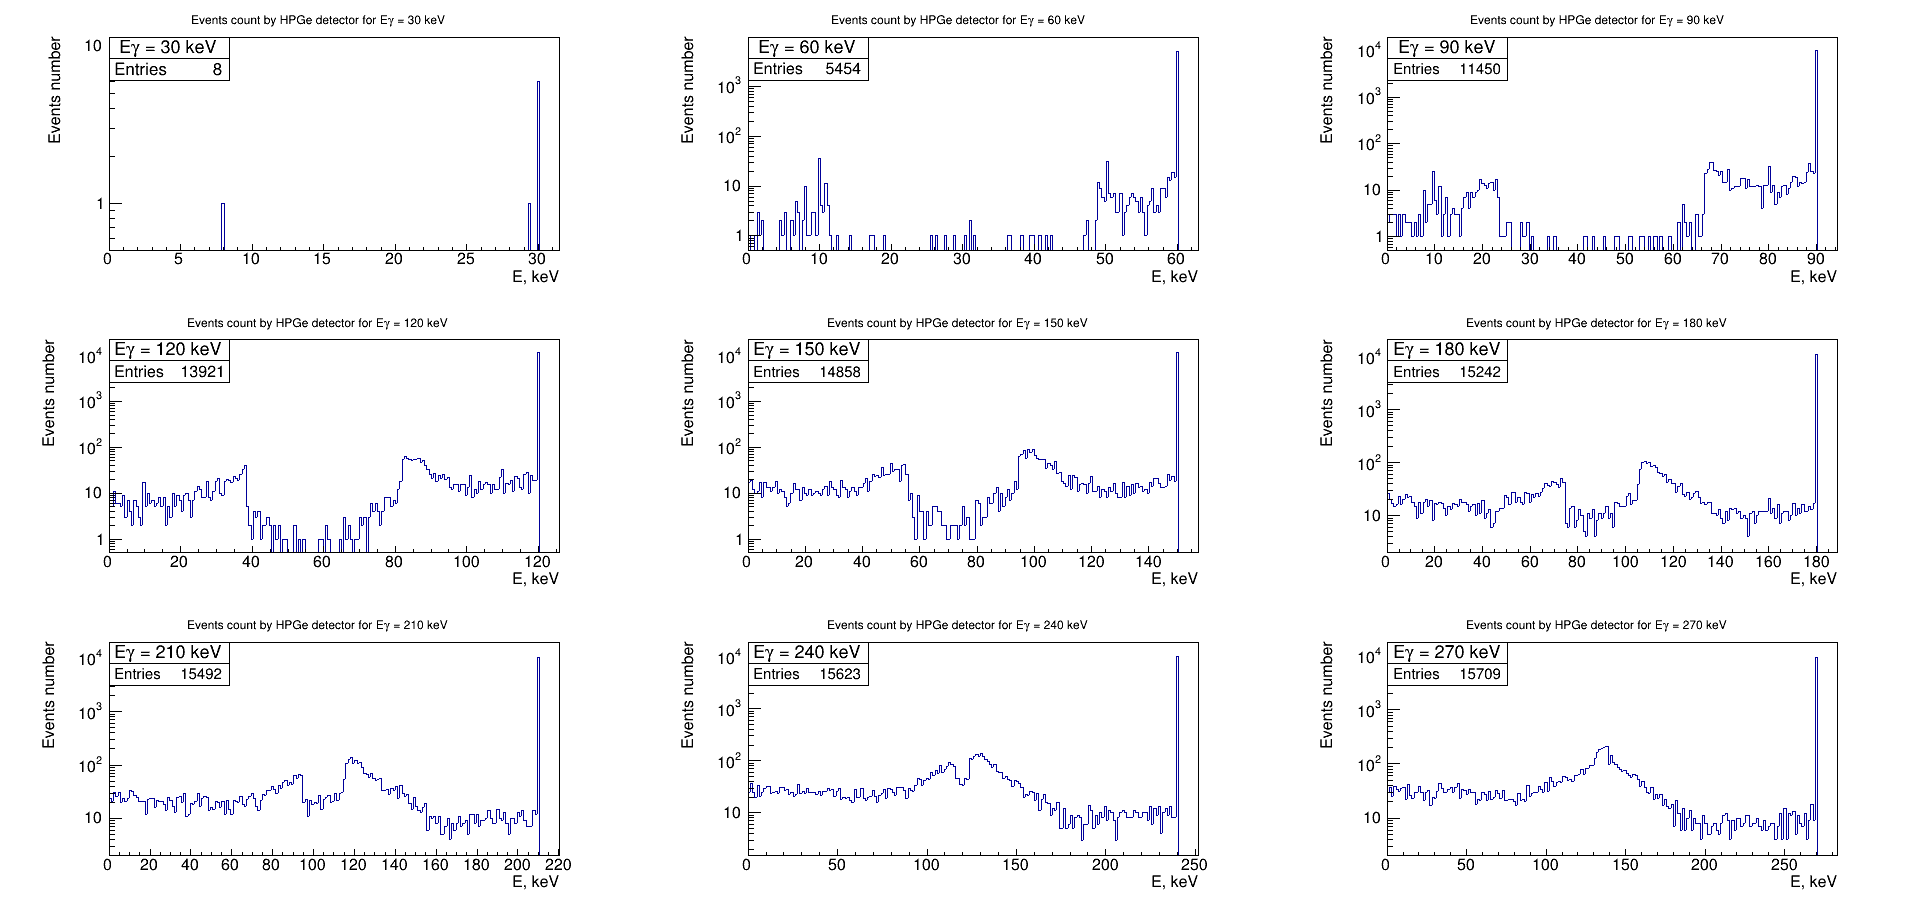
\includegraphics[width =\textwidth]{images/Gamma30-270.png}
    \caption{Спектры зарегистрированных событий для малых энергий гамма-кванта}
    \label{fig:my_label}
\end{figure}


\begin{figure}
    \centering
    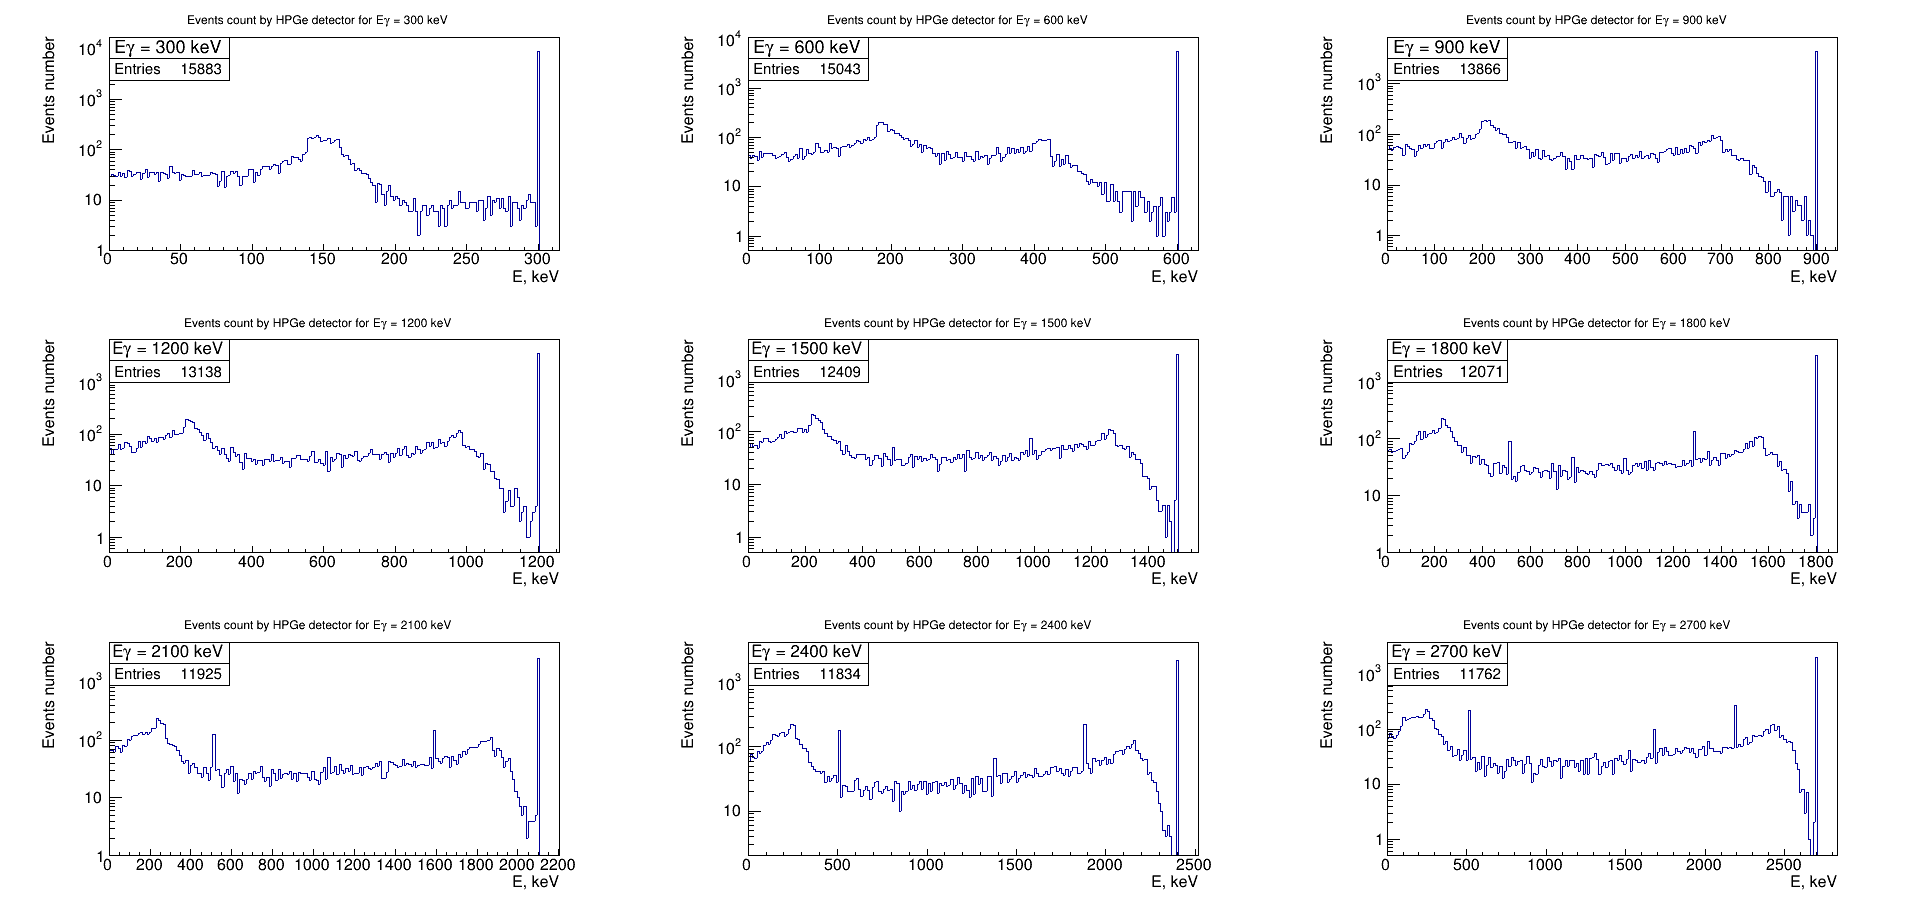
\includegraphics[width =\textwidth]{images/Gamma300-2700.png}
    \caption{Спектры зарегистрированных событий для высоких энергий гамма-кванта}
    \label{fig:my_label}
\end{figure}

Чувствительность детектора вычислялась как отношение зарегистрированных событий в пике к полному числу выпущенных частиц:

\begin{figure}
    \centering
    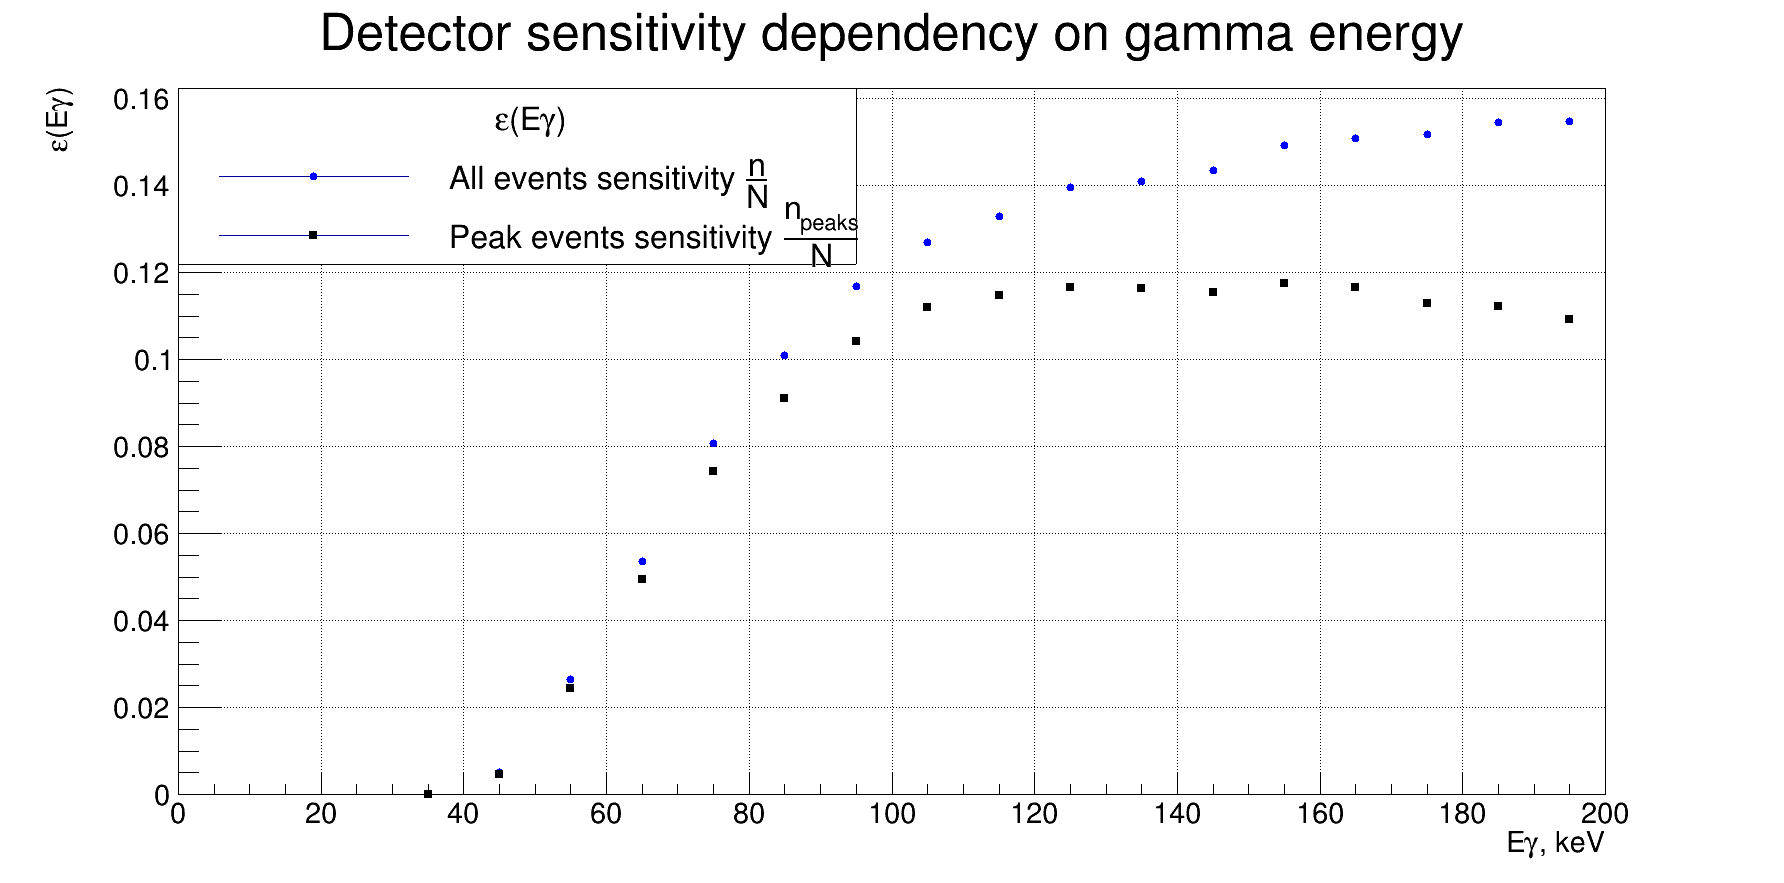
\includegraphics[width =\textwidth]{images/epsilon0-200.png}
    \caption{Чувствительность детектора в диапазоне малых энергий гамма-кванта}
    \label{fig:my_label}
\end{figure}

\begin{figure}
    \centering
    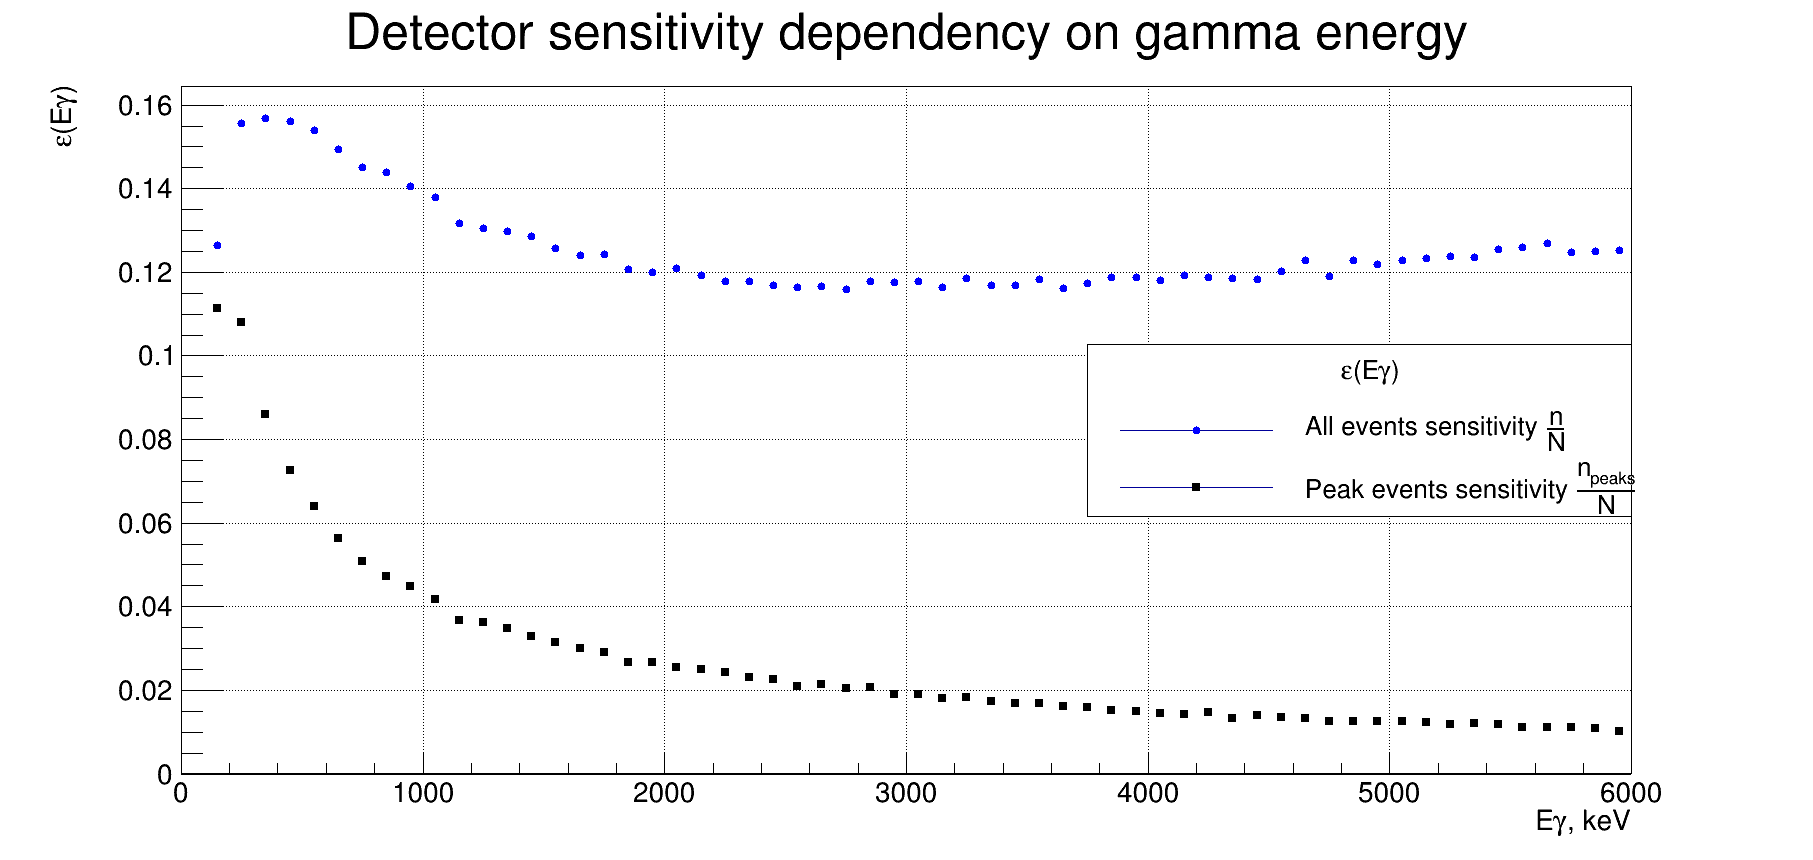
\includegraphics[width =\textwidth]{images/epsilon0-6000.png}
    \caption{Чувствительность детектора в диапазоне энергий естественного радиационного фона}
    \label{fig:my_label}
\end{figure}

\subsection{Экспериментальные спектры сырья}
    
    TODO(есть, но их нужно калибровать)
    
\subsection{Верхний предел на содержание}
     TODO

\section{Верхний предел на существование аксиона}

\subsection{Моделирование эксперимента}
Эксперимент моделировался на Geant4 следующим образом:
TODO
\subsection{Оценка числа возможных аксионных событий}
Slim < чего-то

\subsection{Предел на константы связи}
Найдём число ядер в мишени ${N_{Tm}}$ Для этого вычислим молярную массу вещества детектора:
\begin{equation}
    \mu \left( {T{m_3}A{l_5}{O_{12}}} \right) = 3 \cdot 168.93 + 5 \cdot 26.98 + 12 \cdot 16 = 833.69\frac{\text{г}}{{\text{моль}}}
\end{equation}

Каждая молекула мишени содержит 3 ядра $^{169}Tm$, поэтому

\begin{equation}
    N_{Tm} = 3\nu  \cdot {N_A} = 3\frac{m}{\mu }{N_A} = 3\frac{m}{\mu }{N_A}
\end{equation}

Подставляя $m=
8.18 \text{ г}$, получаем ${N_{Tm}} = 3 \cdot \frac{{8.18}}{{833.69}} \cdot 6.022 \cdot {10^{23}} \approx 1.77 \cdot {10^{22}}$


Полное число зарегистрированных событий в пике, который можно сопоставить с аксионом, пропорционально числу ядер $^{169}Tm$ в мишени, времени измерений и эффективности регистрации детектором. Вероятность зарегистрировать аксионный пик зависит от уровня фона и разрешения детектора. Полагая:
\begin{itemize}
    \item Число ядер в мишени $N_{Tm} = 1.77 \cdot {10^{22}}$
    \item Эффективность регистрации $\varepsilon \sim 1 $, так как в болометрических детекторах ядра мишени находится непосредственно внутри активного объема
    \item Время экспозиции 1 год: $T = 3.15 \cdot {10^7} c$
\end{itemize}

Мы можем записать предел:
\begin{equation}
   \varepsilon  \cdot T \cdot {R_A} \cdot N_{Tm} \leqslant {S_{\lim }}
\end{equation}

Если предположить $\frac{{{p_A}}}{{{p_\gamma}}} \approx 1$, то можно получить ограничение на константы связи, воспользовавшись выражением \eqref{RAg}:

\begin{equation}
     \left| g_{A\gamma}^2{\left( {g_{AN}^0 + g_{AN}^3} \right)^2} \right| \leqslant \frac{{S_{\lim }}}{{C_{Ax}} \cdot \varepsilon  \cdot T \cdot N_{Tm} } 
\end{equation}


\begin{equation}
     \left| g_{Ae}^2{\left( {g_{AN}^0 + g_{AN}^3} \right)^2} \right| \leqslant \frac{{S_{\lim }}}{{C_{Ae}} \cdot \varepsilon  \cdot T \cdot N_{Tm} } 
\end{equation}

\newpage

\specialsection{Выводы}
Проведённые расчёты показывают, что создание криогенной установки на основе тулиевых болометров может улучшить существующие экспериментальные пределы на несколько порядков
\pagebreak

\specialsection{Заключение}
Основные результаты, полученные в работе, заключаются в
следующем:
1. Создана экспериментальная установка с Si(Li)-детекторами и
мишенью из 169Tm. Низкофоновая установка включает в себя пассивную и
активную защиту от космического излучения, а также регистрирующую
аппаратуру.
2. Создана программа накопления данных с Si(Li)-детекторов,
позволяющая проводить длительные измерения и контролирующая работу
детекторов и активной защиты. Создана программа для расчета
эффективности регистрации гамма-квантов для различной геометрии между
планарным детекторам и мишенью.
3. Проведен поиск резонансного поглощения солнечных аксионов,
возникающих в результате конверсии тепловых фотонов в поле плазмы,
ядрами 169Tm, приводящего к возбуждению первого ядерного уровня  соответствующий энергии первого
возбужденного уровня 169Tm, статистически не проявился, что позволило

Полученные результаты были представлены на 146 международной
конференции по проблемам ядерной спектроскопии и структуре атомного
ядра (Кибердянск 2077) и опубликованы в работах



% Библиография в cpsconf стиле
% Аргумент {1} ниже включает переопределенный стиль с выравниванием слева
\begin{thebibliography}{1}
\bibitem{voc} Griffin D.W., Lim J.S. \flqq Multiband excitation vocoder\frqq. IEEE ASSP-36 (8), 1988, pp. 1223-1235.
\bibitem{vo2} Griffin D.W., Lim J.S. \flqq Multiband excitation vocoder\frqq. IEEE ASSP-36 (8), 1988, pp. 1223-1235.
\end{thebibliography}
\end{document}